\documentclass[output=paper]{langsci/langscibook}  
\author{Dakota J. Thomas-Wilhelm\affiliation{University of Iowa; Universitat Autònoma de Barcelona}\lastand Carmen Pérez-Vidal\affiliation{Universitat Pompeu Fabra} }
\title{Exploring the acquisition of countable and uncountable nouns in English-medium instruction and formal instruction contexts}
\shorttitlerunninghead{Exploring the acquisition of (un)countable  nouns in EMI and FI contexts}
 
 
\abstract{The present study aims to explore the acquisition and mental representation of the countable and uncountable noun distinction in English as a foreign language (EFL) by two upper-intermediate Catalan/Spanish groups in two different learning contexts, formal instruction (FI) and English-Medium Instruction (EMI) (\citealt{Coleman2006}; \citealt{Izumi2013}), in contrast with baseline native speaker data, and with an interest in crosslinguistic influence. The FI group receives fewer hours of exposure to EFL, 3 per week, but in return, instruction on the phenomenon under study. In contrast, the EMI group is immersed in EFL, receiving 15-20 hours per week in the classroom, but receives no instruction on the phenomenon in question. Data were collected by means of two experimental tasks: one grammaticality judgment task and one picture-decision task. The results show that, although there is no significant difference between learning context overall, there are differences when the data are considered at the level of the noun-type. The lack of impact resulting from FI adds further evidence to the existing discussion related to explicit (FI) versus implicit (EMI) instructional contexts (\citealt{DafouzGuerrini2009}; \citealt{Pérez-Vidal2009}; \citeyear{Pérez-Vidal2011}). In addition, these findings underscore the difficulty in the acquisition of countable and uncountable noun type distinctions at upper-intermediate levels. }
\maketitle

\begin{document}  


\section{Introduction}

At the intersection of semantics, syntax, and language \isi{acquisition} is ongoing research about how semantics and syntax are related, and an extension of that is the question of how  language learners acquire this relationship. Barner and Snedeker (\citeyear[42]{BarnerSnedeker2005}) pose a very important question: “how [does] the knowledge in one domain facilitate [the] \isi{acquisition} of knowledge in the other?” The relationship between \isi{countable} and \isi{uncountable} nouns is an exemplar of this relationship between semantics and syntax. This study focuses on how \ili{English} as a Foreign language (\isi{EFL}) learners from two different language \isi{acquisition} contexts, Formal Instruction (\isi{FI}) and \ili{English}-Medium Instruction (\isi{EMI}), acquire \isi{countability} distinctions in their \isi{target language} using both behavioral and cognitive data, with a Grammaticality Judgment Test (\isi{GJT}) and a Picture Decision Task (PDT), respectively (\citealt{Chaudron2003}; \citealt{NorrisOrtega2003}). The study presented in this chapter seeks to understand how \isi{EFL} learners from each context comparatively recognize the \isi{countable}/\isi{uncountable} distinction and map it in their mental representations. 

The study was conducted at a \ili{Catalan} university in Spain where most of the subjects are taught in either \ili{Spanish} or \ili{Catalan}. However, following a relatively recent trend in Europe, \ili{English} has increasingly become a third or additional language of instruction. Indeed, the so-called university \isi{EMI} programs, modeled on similar programs existing at lower stages of education, have become current practice. \citet{WächterMaiworm2014} conducted a survey during the 2006/07 academic year to determine the number of \isi{EMI} programs in the European Higher Education Area. Through their survey, they were able to identify 2,389 programs that were taught though \ili{English}. These findings are remarkable and even more so as the trend was confirmed by a subsequent survey showing that 6\% of degrees in Europe take an \isi{EMI} approach (\citealt{WächterMaiworm2014}). 


\section{Literature review}

Expressing quantity is something that is common in every language. Although it is more complex and developed in some languages than others, nouns, noun phrases, and quantifiers/quantification all have very specific positions and functions in language that allow us to refer to things in both the real and abstract worlds. As can be seen in \tabref{tab:thomas:1}, \ili{English} has five main subclasses of nouns that can refer to objects and substances with physical existence (\citealt{LeechSvartvik1975}): (1) proper, (2) \isi{countable}, (3) object-\isi{uncountable}, (4) substance-\isi{uncountable}, and (5) flexible. In the current study, we are only concerned with subclasses (2)-(5).

\begin{table}
\caption{Noun subclasses in English}
\label{tab:thomas:1}
\small
\fittable{
\begin{tabular}{l lllll}
\lsptoprule 
{} & 
  \bfseries (1) Proper &
  \bfseries (2) Countable & 
  \parbox[t]{20mm}{\raggedright\bfseries (3) Object-uncountable} & 
  \parbox[t]{23mm}{\raggedright\bfseries (4) Substance-uncountable} & 
  \bfseries (5) Flexible\\
\midrule
{I see…} & ~John & *bottle & ~furniture & ~salt & ~cake\\
\tablevspace
& *the John & ~the bottle & ~the furniture & ~the salt &  ~the cake\\
\tablevspace
& *a John & ~a bottle & *a furniture & *a salt & ~a cake\\
\tablevspace
& *some John & *some bottle & ~some furniture & ~some salt & ~some cake\\
\tablevspace
& *Johns & ~bottles & *furnitures & *salts & ~cakes\\ 
\lspbottomrule
\end{tabular}
}
\end{table}

In \ili{English}, \isi{countable} nouns refer to \isi{countable} items and carry the semantic feature of [\textsc{+ count}] (and presumably [\textsc{+ neat}]). On the contrary, \isi{uncountable} nouns refer to non-\isi{countable} items with the semantic feature [– \textsc{count}], and may be [+ \textsc{neat}] or [– \textsc{neat}]. According to \citet{Landman2011}, a noun is [+ \textit{neat}] if the interpretation of its structures does not have \isi{overlapping minimal building} blocks (e.g. \textit{furniture} is comprised of \textit{tables}, \textit{chairs}, \textit{sofas}, whereas a collection of just \textit{tables} would not be considered \textit{furniture}), and a noun is [– \textsc{neat}] if it is comprised of multiple and similar parts which overlap (e.g. \textit{salt} is comprised of multiple, and similar, \textit{grains of salt}). On the basis of such a distinction, \isi{uncountable} nouns are further divided into object-\isi{uncountable} and substance-\isi{uncountable}. Object-\isi{uncountable} nouns are the nouns which are composed of objects (e.g. \textit{furniture, mail, luggage}) and carry the semantic features [\textsc{– count, + neat}], making them “neat” \isi{uncountable} nouns since their interpretation does not have \isi{overlapping minimal building} parts. On the other hand, substance-\isi{uncountable} nouns (“messy” \isi{uncountable} nouns) are those which have the semantic features [\textsc{– count, – neat}] and are composed of substances (e.g. \textit{salt, toothpaste, milk}), whose minimal building parts overlap.  Lastly, flexible nouns are those which can be used as either \isi{countable} [\textsc{+ count}]or \isi{uncountable} nouns [\textsc{– count}] (e.g. \textit{chocolate/chocolates}). In this respect, it is important to note that in the present study, we follow \citet{BarnerSnedeker2005} in positing that the interpretation of flexible nouns as one or the other is driven by the syntax in which they occur, i.e. in \isi{countable} or \isi{uncountable} syntactic constructions. This means that a \isi{flexible noun} will be interpreted as either \isi{countable} or \isi{uncountable} given the context in which it appears. For example, if we compare the sentences \textit{I like chocolate} and \textit{She gave me two chocolates}, the quantifier \textit{two} in the latter sentence drives the interpretation of the \isi{flexible noun} \textit{chocolate} to being \isi{countable}, while the use of the zero article, no quantifier, and singular form of the noun \textit{chocolate} drives the interpretation to be substance-\isi{uncountable} in \textit{I like chocolate}, in the same way that \textit{salt} is \isi{uncountable} in the sentence \textit{I need salt for my fries}.

\ili{Spanish}, \ili{Catalan} and \ili{English} largely overlap in the way they treat \isi{countable} and \isi{uncountable} nouns. Indeed, in the three languages \isi{countable} nouns (like \textit{chair}) refer to \isi{countable} items and mass-\isi{uncountable} nouns (like \textit{water}) denote non-\isi{countable} items (\citealt{Bruyne1995}; \citealt{WheelerEtAl1999}; \citealt{ButtBenjamin2004}). The important difference is that some nouns that are treated as object-\isi{uncountable} in \ili{English} (thus appearing in the singular only in this language),  in \ili{Spanish} and \ili{Catalan} have both a singular and plural form, expressing two different meanings. As can be seen in Tables 2 and 3, in \ili{Spanish} or \ili{Catalan} the singular form indicates an unspecified mass, while its plural refers to a plurality of objects; to express this meaning, \ili{English} requires the addition of words that are \isi{countable} elements. This is an important difference because one might expect that native speakers (\isi{NSs}) of \ili{Spanish} and \ili{Catalan} might try to pluralize \ili{English} \isi{uncountable} nouns in trying to achieve the meaning that is similarly expressed in \ili{Spanish} and \ili{Catalan}.
 
\begin{table}
\caption{{Pluralizing Spanish uncountable nouns}}
\label{tab:thomas:2}

\begin{tabularx}{\textwidth}{XXXX}
\lsptoprule
\multicolumn{2}{c}{\bfseries SINGULAR} & \multicolumn{2}{c}{\bfseries PLURAL}\\
\ilit{Spanish} & \ilit{English} & \ilit{Spanish} & \ilit{English}\\
\midrule 
pan & \textit{bread} & panes & \textit{loaves of bread}\\
tostada & \textit{toast} & tostadas & \textit{pieces of toast}\\
equipaje & \textit{luggage} & equipajes & \textit{pieces of luggage}\\
basura & \textit{garbage} & basuras & \textit{bags of garbage}\\
\lspbottomrule
\end{tabularx}
\end{table}

\begin{table}
\caption{Pluralizing Catalan uncountable nouns}
\label{tab:thomas:3}

\begin{tabularx}{\textwidth}{XXXX}
\lsptoprule
\multicolumn{2}{c}{\bfseries SINGULAR} & \multicolumn{2}{c}{\bfseries PLURAL}\\
\ilit{Catalan} & \ilit{English} & \ilit{Catalan} & \ilit{English}\\
\midrule 
pa & \textit{bread} & pans & \textit{loaves of bread}\\
torrada & \textit{toast} & torrades & \textit{pieces of toast}\\
equipatge & \textit{luggage} & equipatges & \textit{pieces of luggage}\\
basura & \textit{garbage} & basures & \textit{bags of garbage}\\
\lspbottomrule
\end{tabularx}
\end{table}

In developmental research, many hypotheses 
have been discussed 
about how children are sensitive to syntactic information when acquiring nouns that refer to collections of things in \ili{English} (\citealt{BloomKeleman1995}). In the following paragraphs, we will describe the hypothesis put forth by  \citet{BarnerSnedeker2005} and argue for how it may also apply to \isi{foreign language} \isi{acquisition}. 

\citet{BarnerSnedeker2005} presented adults and 4-year old children with pictures and actual scenes, respectively, and asked the question \textit{Who has more?} One of the stimuli contained one or two large objects, the other three or six smaller objects, whose combined mass was clearly smaller than that of the former object(s) (see \figref{fig:thomas:2} for an example). All four classes of nouns addressed in the present study were tested, viz. \isi{countable}, object-\isi{uncountable}, substance-\isi{uncountable}, and flexible.

Results show that, quite expectedly, both children and adults base their judgments on volume, or mass, for substance-\isi{uncountable} nouns (e.g. a large chunk of \textit{toothpaste} is perceived as being ‘more’ than three small ones), and on number for \isi{countable} nouns (e.g. three or six small \textit{shoes} are interpreted as ‘more \textit{shoes}’ than one or two big ones). The crucial finding was that both children and adults use number rather than mass in their judgments of object-\isi{uncountable} nouns. Thus, three small \textit{chairs} and three small \textit{tables} are seen as being ‘more \textit{furniture}’ than a big table with a big chair. It thus seems that the inherent semantics of a word/concept like \textit{furniture} (which denotes a set of individual objects) overrides the lexico-syntactic constraints posed by a given language like \ili{English}, which treats it as an \isi{uncountable} noun like \textit{water}. 

However, syntax does play a role in the case of flexible nouns, like \textit{string}. Here, a plural \isi{syntactic context} like \textit{Who has more strings?} causes most participants to choose the picture with several small pieces of string, whereas a singular \isi{syntactic context} like \textit{Who has more string?} led to choosing the picture with one long piece of string. 

Thus, ‘\isi{individuation}’, i.e. the interpretation of a term as referring to an individual or a collection of individuals, can have at least three sources: inherent semantics, or world knowledge (the fact that furniture or silverware represent, in the real world, a collection of objects); lexical features (the fact that, at least in \ili{English}, ‘furniture’ and ‘silverware’ are singular-only nouns); and \isi{syntactic context} (e.g. the presence of quantifiers and plural morphology, in the case of flexible nouns). 


\section{Methodology}

These are the research questions addressed in the current study: 

\begin{itemize}
\item[\textbf{RQ1.}] How do \isi{FI} learners compare to \isi{EMI} learners, and to \isi{NSs}, in their ability to grammatically recognize different \isi{countable}/\isi{uncountable} noun distinctions?

\item[\textbf{RQ2.}] Are participants’ judgments about quantity based on \isi{linguistic} knowledge or non-\isi{linguistic} world knowledge, and is there any difference in this regard among \isi{FI} and \isi{EMI} learners and native \ili{English} speakers? 
\end{itemize}

\subsection{Participants}


A total of 57 participants completed the two experiments included in this study in order to address our two research questions. Of the 57 participants, 33 were undergraduates completing language-specialty degrees (\isi{FI} group) and 24 were undergraduates studying business-related degrees through \ili{English} (\isi{EMI} group). These two groups were chosen because the \isi{FI} undergraduates received \isi{explicit instruction} in the \ili{English} language, while the \isi{EMI} only received implicit instruction since the content of their courses was taught through the medium of \ili{English}. All participants were \ili{Spanish}/\ili{Catalan} simultaneous bilinguals from a public university in Catalonia, Spain. All participants were controlled for their level of \ili{English}, on the basis of the Cambridge Online Placement Test of \ili{English}. The group represented a relatively homogeneous population having an intermediate level, that is a B.1.2 according to the Common European Framework of Reference. However, results from this test revealed that the \isi{FI} group had a relatively lower level (\textit{M} = 17.55, \textit{SD} = 3.80) than the \isi{EMI} group (\textit{M} = 18.38, \textit{SD} = 0.57). As can be seen by the standard deviations, the \isi{FI} group had considerable variation in level. An independent samples \textit{t}{}-test found that there was no significant difference in the \ili{English} test scores for \isi{EMI} and \isi{FI} contexts (\textit{t}(34) = -1.235, \textit{p} = .225).

In terms of target\isi{language exposure}, there are two main differences between the \isi{EMI} and the \isi{FI} group. Firstly, the students receiving \isi{EMI} received more hours per week of \ili{English} \isi{language exposure} than the \isi{FI} group. The \isi{EMI} group was receiving all of their degree classes, at the time of the study, via \isi{EMI}, which involved between 15-20 hours per week, according to the academic term. In contrast, the \isi{FI} group only had a handful of classes that used \ili{English}, for about  three hours per week. Secondly, the \isi{FI} class hours, as already mentioned, dealt with grammar and linguistics, and, most importantly, included instruction on the phenomenon in focus in this chapter, as part of their established syllabus. Such instruction was not extensive: it included one two-hour session and some homework practice amounting to another two hours, hence four hours in total. In contrast, the \isi{EMI} instructional context had no explicit grammar instruction or attention to form and no specific training on \isi{countability}. In other words, the language and grammar practice that students may obtain in this instructional environment is implicit, which, on its own, is not considered to lead to the same amount of progress as the combination of explicit and implicit teaching conditions \citep{Ellis2010}. In sum, our groups show an interesting contrast: the \isi{EMI} has more contact hours than the \isi{FI} (15-20 hours vs. 3 hours per week); the \isi{FI} has \isi{explicit instruction} on \isi{countability}, which \isi{EMI} does not have. 

A control group (\textit{N} = 26) was also recruited and established for baseline data for the study. These \isi{NSs} came from various \ili{English}-speaking countries, speaking different world Englishes: American \ili{English} (\textit{N} = 18), Canadian \ili{English} (\textit{N} = 4), British \ili{English} (\textit{N} = 3), and  {Australian English} (\textit{N} = 1).  


\subsection{Data collection instruments and procedure}


The data collection was carried out by means of two instruments: a Grammaticality Judgment Task (\isi{GJT}), administered only in \ili{English} (Experiment 1), and a Picture Decision Task (PDT) that was administered in \ili{English}, \ili{Spanish}, and \ili{Catalan} (Experiment 2), respectively. Regarding RQ1, the \isi{GJT} was chosen to provide insight into the participants’ explicit knowledge of the grammaticality of \isi{countable}, \isi{uncountable}, and flexible nouns in different syntactic contexts. Regarding RQ2, a PDT was chosen following the work by \citet{BarnerSnedeker2005}.

 GJTs have been used extensively in second language \isi{acquisition} research and have been determined to be reliable and valid instruments for gathering insight into participants’ explicit knowledge of the grammaticality of noun types in different syntactic contexts (e.g. \citealt{CowanHatasa1994}; \citealt{Gass1994}; \citealt{Cowart1997}; \citealt{IoninZyzik2014}, among others). In the present study, the \isi{GJT} was administered in \ili{English} only and  consisted of 100 sentences which the participants had to individually rate based on whether each sentence sounded linguistically \isi{grammatical} to them. For each item, participants had to choose one of the following options: \textit{very natural – natural – not natural – not natural at all}.\footnote{In order to avoid forcing the non-native speakers (\isi{NNSs}) of \ili{English} to choose between two extreme options (\textit{very natural}/\textit{not natural at all}), we decided to include the intermediate values \textit{natural} and \textit{not natural}, although the distinctions between \textit{very natural}/\textit{natural} and \textit{not natural}/\textit{not natural at all} were not taken into an account because of the decision to use a right-wrong approach for data analysis.} Participants were required to give a judgment on each of the 100 items. A sample item from the \isi{GJT} can be found in \figref{fig:thomas:1}.

\begin{figure}[t]
\fbox{\parbox{.9\textwidth}{\centering
\textit{There are many furnitures to choose from.}
\begin{itemize}
\item very natural
\item natural
\item not natural
\item not natural at all
\end{itemize}
}}
\caption{\label{fig:thomas:1} A sample item from the GJT}
\end{figure}

 
As can be seen in \figref{figtab:thomas:4}, \isi{GJT} target sentences were created based on the five \isi{different noun} types (\isi{countable}, object-\isi{uncountable}, substance-\isi{uncountable}, [\textsc{– count}] flexible, and [\textsc{+ count}] flexible). After consulting  specialists in both semantics and \isi{pragmatics} of \ili{Spanish}, \ili{Catalan}, and \ili{English},\footnote{Upon consulting with specialists in both semantics and \isi{pragmatics} of \ili{Spanish}, \ili{Catalan}, and \ili{English}, which allowed us to determine the crosslinguistic status, two conditions were created in order to devise the tokens for testing.} two \textit{crosslinguistic statuses} were created. The nouns which acted and were used the same in all the languages were considered as the \textit{match} condition, while those which differed between languages were considered the \textit{mismatch} condition. The only category that consisted of mismatched tokens was object-\isi{uncountable}. This created a total of five conditions. All items were presented in both \isi{grammatical} and ungrammatical sentences. Overall, there were 50 experimental sentences and 50 fillers (25 \isi{grammatical} and 25 ungrammatical).

% %%please move \begin{table} just above \begin{tabular . 
% \begin{table}
% \caption{Conditions for items in the GJT}
% \label{tab:thomas:4}
% 
% \begin{tabularx}{\textwidth}{XXrlQ}
% \lsptoprule
% 
% {\bfseries Noun type} & \bfseries Crosslinguistic status & \bfseries \# & \bfseries Grammaticality & \bfseries Example item\\
% \midrule 
% {Countable} & match & 4 &grammatical & \textit{You have many books.}\\
% \hhline{~~---} 
% &  & 4 & ungrammatical & \textit{There is a lot of book on the table.}\\
% \midrule
% {Substance-uncountable} & match & 7 &grammatical & \textit{I like salt on my potatoes.} \\
% \hhline{~~---} 
% &  & 3 & ungrammatical & \textit{The salts are on the table.}\\
% \midrule
% \multirow{4}{2cm}{~\newline~\newline~\newline Object-\newline uncountable} & match & 4 &grammatical & \textit{That is beautiful cutlery.}\\
% \hhline{~~---} 
% &  & 4 & ungrammatical & \textit{These cutleries are from Italy.}\\
% \hhline{~~---} 
% & mismatch & 4 &grammatical & \textit{I had quite a bit of toast for breakfast.}\\
% \hhline{~~---} 
% &  & 4 & ungrammatical & \textit{She will have two toasts with her breakfast.}\\
% \midrule
% {Flexible\newline [\textsc{+ count}]} & match & 4 &grammatical & \textit{John put three cakes on the counter.}\\
% \hhline{~~---} &  & 4 & ungrammatical & \textit{There is much cakes leftover.}\\
% \midrule
% {Flexible\newline [\textsc{– count}]} & match & 4 &grammatical & \textit{John likes to eat cake.}\\
% &  & 4 & ungrammatical & \textit{There is many cake on the table.}\\
% \hhline{~~---}
% \lspbottomrule
% \end{tabularx}
% \end{table}

\begin{figure}
\caption{Conditions for items in the GJT\label{tab:thomas:4}}
\label{figtab:thomas:4}
\resizebox{!}{20em}{\begin{forest} 
where n children=0{tier=word}{},
    for tree={
	anchor=west,reversed,
	delay={where content={}{shape=coordinate}{}},
        grow'=0, 
        forked edges, 
        align=left
    }
[,l sep=0pt 
[\bfseries\sffamily Noun type,no edge, l=0 [\bfseries\sffamily Crosslinguistic\\\bfseries\sffamily status,tier=match,no edge, l=0 [\bfseries\sffamily {~\#},tier=num,no edge, l=0 [\bfseries\sffamily Grammaticality,no edge, l=0 [\bfseries\sffamily Example,no edge, l=0]]]]]
[{Countable} ,no edge,l=0
  [match, tier=match
    [~4,tier=num
      [grammatical, no edge
	[{\itshape You have\\\itshape  many books.}]
      ]
    ]
    [~4,tier=num
      [ungrammatical, no edge
	[{\itshape There is a lot of\\\itshape  book on the table.}]
      ]
    ]
  ]
]
[{Substance-\\unountable} ,no edge,l=0
  [match, tier=match
    [~7,tier=num
      [grammatical, no edge
	[{\itshape I like salt\\\itshape  on my potatoes.}]
      ]
    ]
    [~3,tier=num
      [ungrammatical, no edge
	[{\itshape The salts are\\\itshape  on the table.}]
      ]
    ]
  ]
]
[{Object-\\uncountable},no edge,l=0 
  [match, tier=match
    [~4,tier=num
      [grammatical, no edge
	[{\itshape That cutlery\\\itshape  is beautiful.}]
      ]
    ]
    [~4,tier=num
      [ungrammatical, no edge
	[{\itshape These cutleries\\\itshape  are from Italy.}]
      ]
    ]
  ]
  [mismatch, tier=match
    [~4,tier=num
      [grammatical, no edge
	[{\itshape I had quite\\\itshape  a bit of toast\\\itshape  for breakfast.}]
      ]
    ]
    [~4,tier=num
      [ungrammatical, no edge
	[{\itshape She will have\\\itshape  two toasts with\\\itshape  her breakfast.}]
      ]
    ]
  ]
]
[{Flexible\\\relax\textsc{[+count]}},no edge,l=0 
  [match, tier=match
    [~4,tier=num
      [grammatical, no edge
	[{\itshape John put three\\\itshape  cakes on the counter.}]
      ]
    ]
    [~4,tier=num
      [ungrammatical, no edge
	[{\itshape There is much\\\itshape  cakes leftover.}]
      ]
    ]
  ]
]
[{Flexible\\\relax\textsc{[\textminus count]}},no edge,l=0
  [match, tier=match
    [~4,tier=num
      [grammatical, no edge
	[{\itshape John likes to\\\itshape  eat cake.}]
      ]
    ]
    [~4,tier=num
      [ungrammatical, no edge
	[{\itshape There is many\\\itshape  cake on the table.}]
      ]
    ]
  ]
]
]
\end{forest}}
\end{figure}

\largerpage
Of the 50 experimental items, 27 were categorized as \isi{grammatical} and 23 as ungrammatical. This imbalance was based on baseline data provided by the \isi{NSs}, where 100\% of the respondents accepted: \textit{The boss asked me to get him a coffee}, as grammatically acceptable and 84.6\% accepted \textit{I’ll take two sugars in my tea} as grammatically acceptable. For this reason, these two substance-\isi{uncountable} nouns were considered as grammatically acceptable while the other substance-\isi{uncountable} tokens that had the plural –\textit{s} were coded as ungrammatical. In any case, these sentences were excluded from subsequent data analysis. All 100 items in the \isi{GJT} and their answers were programmed into Qualtrics and randomized using the Qualtrics function for advanced randomization. One item was presented at a time. The task took the participants approximately 15 minutes to complete. 

For scoring in the case of the \isi{grammatical} items, a right-wrong approach was taken. When coding the options that were available to participants during the AJT, a participant was awarded +2 points for answering \textit{very natural}, +1 point for \textit{natural}, -1 point for \textit{not natural}, and -2 points for answering \textit{not natural at all} for \isi{grammatical} items and the inverse of the point system was used for scoring the ungrammatical items. If an answer was left blank, it was coded with an X to be excluded from data analysis. As already mentioned, the responses of \textit{very natural} and \textit{natural} were bundled together, as well as \textit{not natural} and \textit{not natural at all}, meaning that two scores of +2 carried that same weight as two scores of +1, which were later calculated into percentages of accuracy based on the grammaticality of the sentences. Mean percentages of accuracy were calculated with respect to the different conditions and classes. These were then made into percentages of accuracy for \isi{grammatical} and ungrammatical items. The percentages of accuracy were used for the data analysis.

The second data collection instrument was the PDT, which was administered in \ili{English}. This instrument provided information on quantificational judgments of \isi{countable}/\isi{uncountable} nouns by the participants. Modeled after the experiment by \citet{BarnerSnedeker2005}, this task sought to elicit quantity judgments (the choice of multiple items over a single item) of \isi{countable} and \isi{uncountable} nouns by non-native speakers (\isi{NNSs}) of \ili{English} belonging to the \isi{FI} or \isi{EMI} conditions, and compare those judgments to \ili{English} \isi{NSs}. Following the research conducted by \citet{BarnerSnedeker2005}, of particular interest was whether they would treat object-\isi{uncountable}, such as \textit{furniture} and \textit{luggage}, and flexible nouns (e.g. \textit{cake}, \textit{string}, \textit{chocolate}) presented in [\textsc{+count}] syntax, as quantifying over individuals, or whether they would treat them as substance-\isi{uncountable} nouns (e.g. \textit{toothpaste}, \textit{salt}, \textit{pepper}) and quantify by mass. This was an important sub-question because of the differences between \ili{Catalan}, \ili{Spanish}, and \ili{English} in regard to some of these nouns. The instrument consisted of 24 items in \ili{English}. A sample PDT item can be found in \figref{fig:thomas:2}.




\largerpage[2]
We administered a PDT in \ili{English} to all groups, in which the following question was asked: \textit{Where is there more…?} Upon seeing two pictures — one large item/group, or three small items/groups as shown in \figref{fig:thomas:2}  — this question forced participants to decide where there \textit{was more} of that noun item. Although \citet{BarnerSnedeker2005} posed the question \textit{Who has more…?} in the framing of their experiment, the present study tested the question: \textit{Where is there more…?}\footnote{It might be argued that this presentation may pose the participants with an ungrammatical sentence, for instance \textit{Where is there more books?} We would like to emphasize here that we chose the use of the question \textit{Where is}, and to not change \textit{is} to \textit{are} when presented with plural items, because in \ili{Spanish}/\ili{Catalan}, there is one word/verb form that accounts for both \textit{there is} and \textit{there are}.}\clearpage\noindent  We changed the question in order to provide the participants a \isi{linguistic} form that had a similar structure throughout all three languages (e.g. \ili{English}: \textit{Where are there more books?} \ili{Spanish}: \textit{¿Dónde hay más libros?} \ili{Catalan}: \textit{On hi ha més llibres?}). This change in wording was made so that the data could be usable in another study that compared \ili{English}, \ili{Spanish}, and \ili{Catalan}. Sample items and conditions for the PDT can be found in \tabref{tab:thomas:5}. The participants always chose from the answers: \textit{left – right – I don’t know – There is the same.} As shown in \figref{fig:thomas:2}, the three small objects always showed a combined volume and surface area smaller than the large object.  This allowed responses based on number to be distinguished from those based on mass or volume. 

\begin{figure}[t]
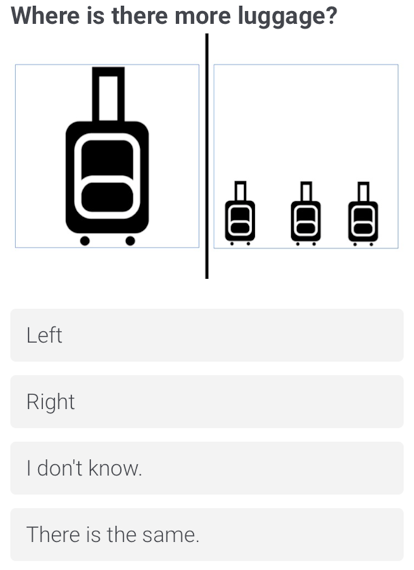
\includegraphics[height=.3\textheight]{figures/thomas-img1.png} 
\caption{\label{fig:thomas:2} A sample item from the PDT}
\end{figure}

\begin{table}
% \todo[inline]{table must be referenced in text}
\caption{Conditions for items in the PDT}
\label{tab:thomas:5}

\begin{tabularx}{\textwidth}{lrQl}
\lsptoprule

\textbf{Noun type} & \textbf{\#} & \textbf{Crosslinguistic status} & \textbf{Example item}\\
\midrule 
Countable & 4 & match & \textit{Where is there more books?}\\

\tablevspace
Substance-\isi{uncountable} & 4 & match & \textit{Where is there more salt?}\\

\tablevspace
\multirow{2}{*}{Object-\isi{uncountable}} & 4 & match & \textit{Where is there more art?}\\
% \hhline{~---} 
& 4 & mismatch & \textit{Where is there more furniture?}\\
% \hhline{~---}

\tablevspace
Flexible [\textsc{+ count}] & 4 & match & \textit{Where is there more cakes?}\\

\tablevspace
Flexible [\textsc{– count}] & 4 & match & \textit{Where is there more cake?}\\
\lspbottomrule
\end{tabularx}
\end{table}

Responses were rated by assigning a +1 if the picture with three small masses or items was chosen and a score of 0 if the picture of one large mass or item was chosen. A score of 0 was also assigned to \textit{They have the same} responses and an X was assigned to \textit{I don’t know}. The X scores were later excluded from data analysis. The scores were calculated and analyzed as percentages of \isi{individuation} (e.g. total number of 1s divided by the total number of that \isi{noun type} presented). In the PDT, as with the \isi{GJT}, target sentences were created based on the five \isi{different noun} types (\isi{countable}, object-\isi{uncountable}, substance-\isi{uncountable}, [\textsc{–count}] flexible, and [\textsc{+ count}] flexible). 

Prior to participating in data collection, the participants completed two pre-participation questionnaires: a biodata and language use questionnaire and a quick \ili{English} test. These questionnaires were web-based for all participants and administered via Qualtrics.\footnote{\url{http://www.qualtrics.com}, accessed 2015/01 -- 2015/06} The \isi{NSs} were sent the information via an email containing links to the experimental tasks, as well as a sociolinguistic survey. They were asked to complete the surveys within three weeks, and those who completed all the tasks were included in the data analysis.  \isi{NNS} participants attended a data collection session in an on-campus computer lab during which they were administered the entire battery of instruments over the course of an hour and a half. The participants were offered a short break of 5-10 minutes between each of the data collection steps. 


\section{Results and discussion}


\subsection{Experiment 1}


Experiment 1 allows us to address RQ1, that is, how the \isi{FI} group would compare to the \isi{EMI} and to \isi{NSs} of \ili{English} in their ability to grammatically recognize \isi{countable}/\isi{uncountable} noun distinctions, including object-\isi{uncountable} noun, substance-\isi{uncountable} nouns, and \isi{flexible noun} types, and whether any influence from their two L1s would be revealed.  In order to address this question, a series of one-way ANOVAs was run on the mean accuracy (scores out of 100) of the \isi{GJT} with an alpha level set at 0.05. For the noun types tested, there was a statistically significant difference between groups as determined by one-way ANOVAs for \isi{countable} nouns (\textit{F}(2,80) = 23.085, \textit{p} < .001), object-\isi{uncountable} nouns (\textit{F}(2,80) = 96.938, \textit{p} < .001), flexible [+ \textsc{count}] nouns (\textit{F}(2,80) = 22.894, \textit{p} < .001), and flexible [– \textsc{count}] nouns (\textit{F}(2,80) = 18.619, \textit{p} < .001). There was no statistical difference between groups for substance-\isi{uncountable} nouns (\textit{F}(2,80) = 1.806, \textit{p} = .171). Average accuracy rates are presented in \tabref{tab:thomas:6}.
 
\begin{table}
\caption{GJT sescriptive statistics}
\label{tab:thomas:6}
\small
\begin{tabularx}{\textwidth}{QYYYYY}
\lsptoprule
\bfseries Group &
\bfseries Countable nouns & 
\bfseries Object-\isi{uncountable} nouns & 
\bfseries Substance-\isi{uncountable} nouns & 
\bfseries Flexible\newline [+ \textsc{count}] nouns & 
\bfseries Flexible\newline [– \textsc{count}] nouns\\
\midrule
\isi{NSs} & 90.88 & 93.27 & {87.00} & {96.15} & 91.35\\
(\textit{n} = 26) & (9.05) & (8.23) & {(15.15)} & {(5.88)} & (9.20)\\
\isi{FI} context & 83.71 & 46.97 & {80.30} & {75.76} & 71.59\\
(\textit{n =} 33) & (19.13) & (11.49) & {(17.50)} & {(17.10)} & (15.40)\\
\isi{EMI} context & 64.84 & 79.17 & {78.13} & {73.44} & 76.69\\
(\textit{n =} 24) & (8.99) & (18.26) & {(19.59)} & {(13.45)} & (11.36)\\
\lspbottomrule
\end{tabularx}
\end{table}

Looking at individual comparisons from a descriptive point of view, results of the \isi{GJT} provided evidence that \isi{L2} \ili{English} learners, from both the \isi{EMI} and the \isi{FI}, showed some difficulty in judging the grammaticality of constructions with \isi{countable} and \isi{uncountable} nouns in comparison to \isi{NSs} of \ili{English}. As visible in \tabref{tab:thomas:6}, the \isi{NSs} performed with rates of accuracy nearly at ceiling across all the classes of nouns, with the exception of substance-\isi{uncountable} nouns. All learner groups  showed accuracy rates lower than those of the NS group in all categories. In \figref{fig:thomas:3}, it can be seen that the \isi{EMI} participants performed, on average, lower than those in a \isi{FI} context with the exception of object-\isi{uncountable} nouns (e.g. \textit{They have such beautiful furniture in their house} or \textit{There are many furnitures to choose from}) and flexible nouns used in a [\textsc{– count}] context (e.g. \textit{John has some string in his bag}). 

\begin{figure} 
% 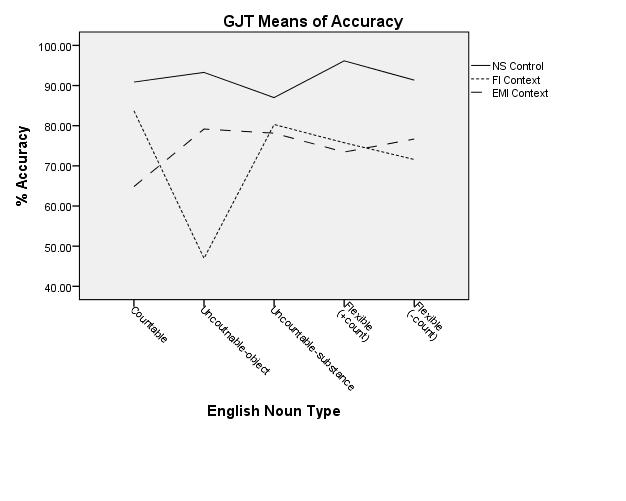
\includegraphics[width=\textwidth]{figures/thomas-img2.jpg}

  \begin{tikzpicture}
    \begin{axis}[
	xlabel={\ili{English} noun type},   
	x label style={at={(axis description cs:0.5,-0.1)},anchor=north},
	ylabel={\% accuracy}, 
	axis lines*=left, 
        width  = .8\textwidth,
	height = .45\textheight,
    	nodes near coords, 
	xtick=data, 
	xticklabel style={rotate=15,anchor=east,yshift=-2.5mm,xshift=2mm}, 
	ymin=40,
	ymax=100, 
	symbolic x coords={countable, uncountable object, uncountable substance, flexible [+count], flexible [–count]},
	legend style={at={(1,0.4)},anchor=west}, 
	] 
	\addplot[draw=lsDarkBlue,thick] 
	    coordinates {(countable,90.86538) (uncountable object,93.26923) (uncountable substance,86.99634) (flexible [+count],96.15385) (flexible [–count],91.34615) };
	\addplot[draw=lsMidGreen,thick, dashed] 
	    coordinates {(countable,83.71212) (uncountable object,46.9697) (uncountable substance,80.30303) (flexible [+count],75.75758) (flexible [–count],71.59091) };
	\addplot[draw=lsMidOrange,thick, dotted] 
	    coordinates {(countable,64.84375) (uncountable object,79.16667) (uncountable substance,78.125) (flexible [+count],73.4375) (flexible [–count],76.69271) };
	\legend{NS control, \isi{FI} context, \isi{EMI} context}
    \end{axis} 
  \end{tikzpicture} 
\caption{\label{fig:thomas:3} Profile plot of the participant groups’ performance on GJT}
\end{figure}


In order to test the significance of these differences among groups, post hoc tests using Tukey HSD were conducted. We will address each of the noun types individually. 

As for \isi{countable} nouns (e.g. judging the grammaticality of \textit{There are six dogs playing in the park} versus \textit{One third of the dog is in the garden}), a Tukey HSD post hoc test revealed that the \isi{FI} learners (\textit{M} = 83.71, \textit{SD} = 19.13) were significantly different (\textit{p} < .001) from the \isi{EMI} learners (\textit{M} = 64.84, \textit{SD} = 8.99). The \isi{FI} learners were not significantly different from the \isi{NSs} (\textit{M} = 90.87, \textit{SD} = 9.05, \textit{p} = .131), while the \isi{EMI} leaners were (\textit{p} < .001). 

For  object-\isi{uncountable} nouns (e.g. \textit{They have such beautiful furniture in their house} vs. \textit{There are many furnitures to choose from}), the \isi{FI} learners' means of accuracy was below 50\% (\textit{M} = 46.97, \textit{SD} = 11.49), which was much lower than the \isi{EMI} learners (\textit{M} = 79.17, \textit{SD} = 18.26). A Tukey HSD post hoc analysis showed that this difference  was significant with \textit{p} < .001. When comparing the \isi{NNSs} to \isi{NSs} (\textit{M} = 93.27, \textit{SD} = 8.83), both learning contexts performed significantly lower (\textit{p} < .001 for both groups). 

In regard to substance-\isi{uncountable} nouns, the \isi{NSs} performed lower than 90\% overall (\textit{M} = 87.00, \textit{SD} = 15.15), and both NNS groups’ accuracy was quite close to this level. Thus, the difference with learner groups was not significant: \textit{p} = .314 for the \isi{FI} learners and \textit{p} = .178 for the \isi{EMI} learners. The \isi{FI} learners were on average slightly more accurate (\textit{M} = 80.30, \textit{SD} = 17.50) than the \isi{EMI} learner group (\textit{M} = 78.13, \textit{SD} = 19.59), although this difference was not significant (\textit{p} = .888). 

\newpage 
The data concerning flexible nouns do not show any relevant differences between the experimental groups. For flexible nouns presented with count syntax, henceforth flexible [\textsc{+ count}], the NS group performed at high rates of accuracy (\textit{M} = 96.15, \textit{SD} = 5.88). The \isi{EMI} learners performed with the lowest mean accuracy (\textit{M} = 73.44, \textit{SD} = 13.45), while the \isi{FI} learners performed a little higher (\textit{M} = 75.76, \textit{SD} = 17.10). The difference between the two experimental groups was not significant (\textit{p} = .796), although they both performed significantly lower than the \isi{NSs} (\textit{p} < .001 for both groups).

Flexible nouns presented in \isi{uncountable} syntax, flexible [\textsc{– count}], present a different picture, with the \isi{EMI} learners achieving slightly higher rates of accuracy (\textit{M} = 76.69, \textit{SD} = 11.36) than the \isi{FI} learners (\textit{M} = 71.59, \textit{SD} = 15.40), although this difference was not significant (\textit{p} = .291). The \isi{NSs} achieved significantly higher rates of accuracy (\textit{M} = 91.35, \textit{SD} = 9.20) than both of the experimental groups (\textit{p} < .001 for both groups). 

To summarize, the first \isi{research question} explored the \isi{linguistic} ability of both the \isi{FI} and \isi{EMI} experimental groups of \isi{NNSs} in comparison to \isi{NSs} in their ability to recognize \isi{grammatical} and ungrammatical uses of \isi{countable}/\isi{uncountable} noun distinctions in \ili{English}. The results of the \isi{GJT} provided evidence that the \isi{NNSs}, both \isi{FI} and \isi{EMI}, showed some difficulty, although not significant in all noun types. In comparison to \isi{NSs}, differences were significant in the case of \isi{countable} nouns for the \isi{EMI} group, for both groups in the case of object-uncount\-ables, and non-significant for substance-\isi{uncountable} and for flexible nouns in \isi{countable} contexts. They were again significant for both groups for flexible nouns in \isi{uncountable} contexts. 

When comparing learning contexts, the \isi{FI} group performed significantly better than the \isi{EMI} group with regard to \isi{countable} nouns, while they performed only slightly higher with substance-\isi{uncountable} nouns and flexible [\textsc{+ count}]. The \isi{EMI} group did perform slightly better than the \isi{FI} group with regard to object-\isi{uncountable} nouns and flexible [\textsc{– count}] nouns.  Thus, there was no clear trend favoring either \isi{FI} or \isi{EMI}. It must be remembered that the \isi{EMI} group had around seven times more hours of exposure per week than the \isi{FI} group (15/20 versus 3, respectively), potentially including many contexts for using these classes of nouns. On the other hand, the \isi{FI} group had received \isi{explicit instruction}, and more precisely 4 hours, on \isi{countability} issues. Consequently, it can be stated that the contrast between both groups in terms of quantity and quality of exposure also results in mixed, or asymmetric, comparative results. 



\subsection{Experiment 2}


 Experiment 2 allows us to address RQ2: to what extent the judgments elicited with the PDT were based on \isi{linguistic} or extra-\isi{linguistic} knowledge and whether there are any differences among \isi{EMI} and \isi{FI} students and L1 \ili{English} speakers.  

We will now look at the results of the PDT in \ili{English} and compare the \isi{EMI} learners to the \isi{FI} learners and the \isi{NSs}. Results will be reported as percentages of \isi{individuation} based on \ili{English} \isi{noun type}. It should be borne in mind that answers were scored by awarding +1 point if the participant chose the picture with three small masses or items and a score of 0 if the picture chosen represented a large mass or item. To calculate percentages of \isi{individuation}, the positive numbers were added together and then divided by the total number of items in that category, which was always 4. In other words, if a participant chose the picture of three small items for \textit{books, dogs,} and \textit{doors}, but not for \textit{windows}, then they would receive a score of 3. That score was then divided by 4 to get a percentage of individuation as 75\%. One would predict lower percentages of \isi{individuation} for uncountable-substance and flexible [\textsc{– count}] items. For example, if a participant selected the picture of three small piles for \textit{cake}, but the larger mass for \textit{paper, stone,} and \textit{chocolate}, then they would receive a score of 1 out of four. That would be converted into a percentage of \isi{individuation} of 25\%. In short, one would expect high percentages of \isi{individuation} for \isi{countable}, object-\isi{uncountable}, and flexible [\textsc{+ count}] nouns since those nouns are \isi{countable} and, therefore, refer to objects that can be individuated and low percentages of \isi{individuation} for substance-\isi{uncountable} and flexible [– count] nouns since those nouns are \isi{uncountable} and, therefore, refer to masses of substances. 

In order to address this \isi{research question}, a series of one-way ANOVAs was run on the mean percentages of \isi{individuation} (scores out of 100) of the PDT, with an alpha value set at 0.05. For the noun types tested, there was no statistically significant difference between groups as determined by one-way ANOVA for \isi{countable} nouns (\textit{F}(2,80) = .029, \textit{p} = .972), object-\isi{uncountable} nouns (\textit{F}(2,80) = 1.181, \textit{p} = .312), or substance-\isi{uncountable} nouns (\textit{F}(2,80) = .189, \textit{p} = .828). As for flexible nouns, there was no statistical difference found for flexible [\textsc{+ count}] nouns (\textit{F}(2,80) = .115, \textit{p} = .892) nor flexible [\textsc{– count}] nouns (\textit{F}(2,80) = .078, \textit{p} = .925). Individuation rates are provided in \tabref{tab:thomas:7}.
 
\begin{table}
\caption{PDT descriptive statistics}
\label{tab:thomas:7}
\small
\begin{tabularx}{\textwidth}{QYYYYY}
\lsptoprule
\bfseries Group & \bfseries Countable nouns & \bfseries Object-\isi{uncountable} nouns & {\bfseries Substance-\isi{uncountable} nouns} & {\bfseries Flexible} 

\bfseries [\textsc{+ count}] nouns & {{\bfseries Flexible}

\bfseries [\textsc{– count}] nouns}\\
\midrule
\isi{NSs} & 96.15 & {85.58} & 33.65 & {93.27} & 52.88\\
(\textit{n} = 26) & (15.32) & {(20.22)} & (42.98) & {(20.69)} & (42.03)\\
\isi{FI} context & 96.21 & {76.52} & 27.27 & {91.67} & 56.82\\
(\textit{n =} 33) & (11.04) & {(25.72)} & (36.10) & {(18.40)} & (38.16)\\
\isi{EMI} context & 96.88 & {81.25} & 30.21 & {93.75} & 54.17\\
(\textit{n =} 24) & (8.45) & {(20.19)} & (40.36) & {(11.06)} & (37.35)\\
\lspbottomrule
\end{tabularx}
\end{table}

Looking at individual comparisons from a descriptive point of view, results of the PDT provided evidence that \isi{L2} \ili{English} learners, from both the \isi{EMI} and the \isi{FI} groups, showed very similar patterns of \isi{individuation} (or qualificational judgments) to \isi{NSs} of \ili{English}.  \tabref{tab:thomas:7} shows the means of \isi{individuation} for all the groups.  

Given the very similar results, post hoc tests using Tukey HSD showed no statistical differences among groups, with all \textit{p} values higher than .715 

These strong similarities among groups deserve some comments. The most striking, and perhaps unexpected, is that regarding object-\isi{uncountable} nouns (e.g. \textit{Where is there more furniture?}). \ili{English} native speakers’ \isi{individuation} rate was the highest (\textit{M} = 85.58), followed by \isi{EMI} learners  (\textit{M} = 81.25) and \isi{FI} learners (\textit{M} = 76.52). This means that, even though in \ili{English} some nouns are \isi{uncountable} only (e.g. \textit{luggage}, which may be grammaticalized as \isi{countable} in \ili{Catalan}/\ili{Spanish}, i.e. \textit{equipajes}), judgments seem to be based in all cases on semantics (the mental representation of individual objects) rather than on grammar (the mass- vs. count-noun distinction). This provides further evidence for \citegen{BarnerSnedeker2005} claim that, for object-\isi{uncountable} nouns, \ili{English} speakers rely more on semantics than on their language’s grammar. 

Another rather unexpected finding was the proportion of participants who selected the individuating option for substance-\isi{uncountable} nouns. Although all groups perceived these stimuli (such as \textit{water}) to refer more to masses rather than to individuals, and thus tended to select the picture with the big object rather than the one with several small ones, about one third of the answers seemed to interpret some of the substance-\isi{uncountable} nouns as being [+ \textsc{individual}] (e.g. \textit{milk} and \textit{water}). This could be attributed to the fact that, in the PDT, the \isi{uncountable} substances which were liquid, appeared as “cups” of those substances and therefore might have been interpreted as [\textsc{+ individual}].

\largerpage[-1]
A similar phenomenon was observed for flexible nouns. While all three groups consistently interpreted flexible nouns in terms of \isi{individuation} in [\textsc{+ count}] syntactic contexts (e.g. \textit{Where is there more cakes?}), in [\textsc{– count}] contexts (e.g. \textit{Where is there more cake?}) about 50\% of the responses individuated (e.g. chose the picture of three small \textit{cakes}), while the other 50\% did not individuate (e.g. chose the picture of one large \textit{cake}). As with the substance-\isi{uncountable} nouns, it is possible that the pictures that represented flexible nouns in the PDT did not provide appropriate interpretations of mass representations (e.g. a large cake instead of three small cakes). Thus, our experiment provides only partial evidence that syntax drives the individualized interpretation of flexible nouns presented in a [\textsc{– count}] context, as was found by \citet{BarnerSnedeker2005}.


\section{Conclusions}
\largerpage
The present study evaluated the \isi{acquisition} of \ili{English} by \ili{Spanish}/\ili{Catalan} speakers from two different \isi{EFL} learning contexts, conventional \isi{FI} and \isi{EMI}, to gauge their respective impact on learners’ \isi{target language} abilities vis-à-vis \isi{countability}. To do so, we followed \citet{BarnerSnedeker2005}, who used a similar PDT to investigate \ili{English}-speaking children’s developmental patterns and adults’ representations of countable-\isi{uncountable} noun semantics, in addition to a \isi{GJT} based on 100 items. No previous studies have investigated this phenomenon in \isi{NNSs}, specifically from a bilingual background, in different learning contexts, \isi{FI} and \isi{EMI}, and with a crosslinguistic perspective. 

Regarding RQ1, which looked into the \isi{EMI} and \isi{FI} participants’ ability to recognize \isi{grammatical} and ungrammatical uses of \isi{countable}/\isi{uncountable} noun distinctions in \ili{English}, the results of the \isi{GJT} provided evidence that the \isi{NNSs} of \ili{English} showed some difficulty, although not significant in all noun types, with regards to the judgments of \isi{countable} and \isi{uncountable} noun distinctions when used in \isi{grammatical} and ungrammatical contexts in comparison to the \isi{NSs}, irrespective of whether they were studying \ili{English} in a \isi{FI} or \isi{EMI} context. Differences with \isi{NSs} were significant in the case of \isi{countable} nouns for the \isi{EMI} group, in favor of the \isi{NSs}, for both the \isi{FI} and the \isi{EMI} groups in the case of uncountable-objects, in favor of the \isi{NSs}. Differences were non-significant for uncountable-substance and for flexible nouns in both \isi{countable} and \isi{uncountable} contexts. There were no clear and consistent differences between the \isi{EMI} and the \isi{FI} groups, which shows that both programs seem to have similar effects on this dimension of language performance, despite their obvious difference as regards amount of input (15-20 vs. 3 hours per week) and instructional approach (implicit vs. explicit).

  
Regarding RQ2, which enquired into the participants’ judgments of \isi{individuation} for \isi{different noun} types, results have shown a large amount of similarity across groups  when comparing the PDT data collected from \isi{NSs} and \isi{NNSs} of \ili{English}. Most importantly, the fact that \ili{English} \isi{L2} learners had similar response patterns as \isi{NSs} regarding object-\isi{uncountable} nouns, which receive different \isi{grammatical} encodings in \ili{English} versus \ili{Catalan}/\ili{Spanish}, supports \citegen{BarnerSnedeker2005} theory that mental representations of object-\isi{uncountable} nouns do represent individual objects, and provide additional evidence that mental representations do not seem to differ across speakers of different languages, regardless of how each language encodes them in the grammar (as \isi{countable} or \isi{uncountable} nouns). Our results also agree with \citegen{BarnerSnedeker2005} conclusion that flexible nouns are interpreted based on the \isi{syntactic context} in which they occur, although in our data the difference between [\textsc{+ count}] and [\textsc{– count}] contexts was not as clear-cut as in their original experiments. 

This chapter and these conclusions do not come without consequences and limitations, though. We do believe that the presentation of the pictures makes the task to some extent unnatural, although this is true of many controlled experimental conditions. We also believe that expanding the research to all levels of learners would give some better insight into the \isi{acquisition} process of \isi{countable} and \isi{uncountable} nouns. 

\section*{Acknowledgments}

We would like to thank Eloi Puig-Mayenco and Jennifer Ament for their help in participant recruitment and data collection, as well as their valuable comments throughout the writing process. In addition, we would also like to thank the anonymous reviewers and series editors for their insightful comments and suggestions throughout the review process. 


\sloppy
\printbibliography[heading=subbibliography,notkeyword=this] 
\end{document}
